\documentclass[12pt]{article}
 \usepackage[margin=1in]{geometry} 
\usepackage{amsmath}
\usepackage[utf8]{inputenc}
%\usepackage[ utf8 ]{inputenc}
\usepackage[magyar]{babel}
\newcommand{\N}{\mathbb{N}}
\newcommand{\Z}{\mathbb{Z}}
\usepackage{t1enc}
\usepackage{listings}
\usepackage{placeins}
\usepackage{caption}
\usepackage{color}

\usepackage{graphicx}
\usepackage{placeins}
\usepackage{float}
\usepackage{subfigure}

\usepackage{indentfirst}
\usepackage[utf8]{inputenc}
\usepackage[T1]{fontenc}
\title{Véletlen fizikai folyamatok, nyolcadik házi feladat}
\author{Horváth Bendegúz}




\begin{document}
\lstset{frame=tb,
  language=python,
  aboveskip=3mm,
  belowskip=3mm,
  showstringspaces=false,
  columns=flexible,
  basicstyle={\small\ttfamily},
  numbers=none,
  numberstyle=\tiny\color{gray},
  keywordstyle=\color{blue},
  commentstyle=\color{dkgreen},
  stringstyle=\color{mauve},
  breaklines=true,
  breakatwhitespace=true,
  tabsize=3
}

\maketitle
\section*{Szimulációk}
A szimulációkat \texttt{python} nyelven készítettem el.
\subsection*{Véletlenszerű hálózat}
A szimulációban egy $N$ csúcsból álló hálózatot egy $N$ elemű vektorban tároltam, a vektor $N_i$-edik elemének az értéke az $i$-edik csúcspont kapcsolatainak száma. 
\begin{lstlisting}
network = [0]

def simulationStep(n, network):
    toConnect = int(random.uniform(0, n))
    network[toConnect] += 1
    network += [1]
    
for i in range(0,100):
    simulationStep(len(network), network)

\end{lstlisting}
0. lépésben a hálózat egy csúcsból állt, értéke 0 volt. A szimulációs lépés ad nekünk egy egyenletes eloszlású vélelenszámgenerátorral egy 0 és a csúcspontok száma közötti egész típusú véletlenszámot, majd hozzákapcsolja az új csúcsot, és megnöveli az értékét eggyel.  A szimuláció végén a hálózatot  a következő módon elemezhetjük:
\begin{lstlisting}
Nk = np.zeros(max(network))
for i in range(len(network)):
    Nk[network[i]-1]+=1
\end{lstlisting}
Ebben az $Nk_i$ értéke az $i+1$ fokszámú csúcsok száma.
Az így kapott eredményeket a következő táblázatbn foglalom össze:
\begin{center}
\begin{tabular}{|c|c|c|}\hline
szimulációs lépés& fokszámok átlaga & legnagyobb fokszám\\ \hline
1000&1.998 &12 \\ \hline
1000&1.998 &12 \\ \hline
1000&1.998&11 \\ \hline
\end{tabular}
\end{center} 
A fokok számának átlagában nincs változás.
 \begin{figure}[H]
\centering     
\subfigure[]{\label{fig:a}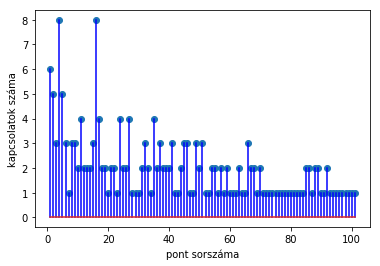
\includegraphics[width=60mm, height = 40mm]{one}}
\subfigure[]{\label{fig:b}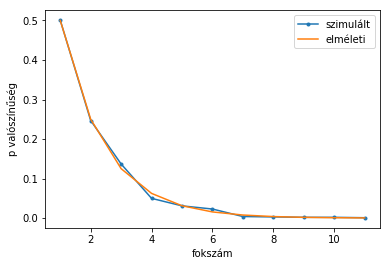
\includegraphics[width=60mm, height = 40mm]{foksz}}
%\subfigure[]{\label{fig:b}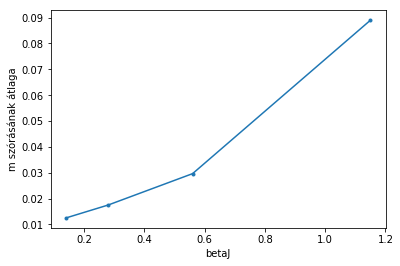
\includegraphics[width = 50 mm,height=35mm]{three}}

\caption{(a) az egyes csúcsokhoz tartozó kapcsolatok száma 100 lépés után(b) a fokszámeloszlás, 1000 lépésből számolva.}
\label{fig: k}
\end{figure}

Az órán számolt végeredmény a fokszámeloszlásra a következő volt:
$$P_k = e^{-k\ln{2}}$$
ezt az elméleti görbét jól követi a szimulációból számolt görbe. Ahhoz, hogy megnézzük, mikor lesz $5\%$-os hibán belül  fokszámeloszlás a következő  módon futtattam a szimulációt:
\begin{lstlisting}
def evalCondition(Nk):
    x = linspace(1, len(Nk), len(Nk))
    state = 0
    tf = True
    a = (exp(-x*log(2))-Nk)/exp(-x*log(2))
    for i in range(min(10, len(Nk))):
        if a[i] < 0.05:
            state += 1
        else:
            state += 0
    if state ==10:
        tf = False
    else:
        tf = True
    return tf
    
network = [0]
a = True
while a:
    simulationStep(len(network), network)
    Nk = np.zeros(max(network))
    for i in range(len(network)):
        Nk[network[i]-1]+=1
    a = evalCondition(Nk)

\end{lstlisting}
 
 Az ebből kapott eredmények:
 \begin{center}
\begin{tabular}{|c|}\hline
szükséges szimulációs lépés\\ \hline
1102 \\ \hline
785 \\ \hline
1211 \\ \hline
727 \\ \hline
870\\ \hline
699 \\ \hline
868 \\ \hline
1620 \\ \hline
1714\\ \hline
\end{tabular}
\end{center} 
A kapott eredmények átlaga: 1066.222, szórása : 358.287, így a szükséges lépések száma $1066.22\pm 358.287$. \\
Az átlagos fokszámot $10^7$ lépés során vizsgáltam, és a 5 tizedes pontossággal $1.99999$-öt adott, így adódik a feltételezés, hogy $lim_{N\to\infty}\langle k\rangle = 2$. Az elméleti számolással a következő módon adódik, használhatjuk $P_k = \frac{1}{2^k}$ diszkrét alakot:
$$\langle k\rangle = \sum^N_kkP_k = \sum^N_k k\frac{1}{2^k} = 2,$$
ha $N\to \infty$.
\newpage
\subsection*{Antipreferenciális hálózat}
A szimulációt úgy valósítottam meg (a feladat szövege szerint), hogyha a kapcsolódás rátájája ($w_k$) kisebb mint egy véletlen $P$ valószínűség, a kapcsolat nem jön létre, nem kerül új csúcs a rendszerbe.
\begin{lstlisting}
def calcNorm(network):
    Nk = np.zeros(max(network))
    for i in range(1, len(network)):
        Nk[network[i]-1]+=1
    a= 0
    for i in range(len(Nk)):
        a+= Nk[i]/(i+1)
    return a    
def calcRates(k, network):
    A = calcNorm(network)
    return 1/A/network[k]
def simulationStep2(network):
    k = int(random.uniform(0,len(network)))
    
    w = calcRates(k, network)
    p = random.uniform(0, 1)
    if p < w:
        network[k] = network[k] + 1
        network += [1]
\end{lstlisting}
Ezáltal sokkal több iteráció kellett, a hálózat egyre lassabban nőtt.
\begin{center}
\begin{tabular}{|c|c|c|}\hline
iteráció&$\langle k\rangle$ & hálózat nagyság \\ \hline
100&1.882352 & 17\\ \hline
1000&1.96153 & 52\\ \hline
10000&1.9854014 &137\\ \hline
100000&1.9954648& 441 \\ \hline
\end{tabular}
\end{center}
A táblázatban látható, hogy $\langle k\rangle$ tart a $2$ felé.


 \begin{figure}[H]
\centering     
\subfigure[]{\label{fig:a}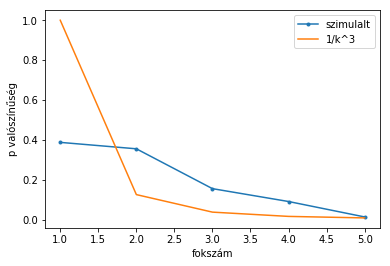
\includegraphics[width=60mm, height = 35mm]{fck}}
\subfigure[]{\label{fig:b}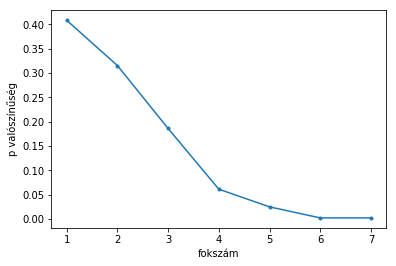
\includegraphics[width=60mm, height = 35mm]{hm}}
%\subfigure[]{\label{fig:b}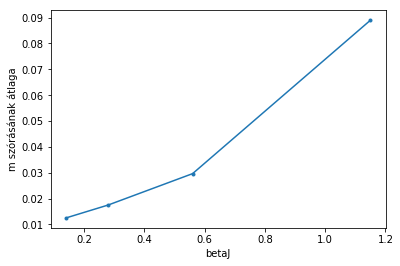
\includegraphics[width = 50 mm,height=35mm]{three}}

\caption{(a) fokszámeloszlás és az $1/k^3$ függvény(b) a fokszámeloszlás, 10000 lépésből számolva.}
\label{fig: k}
\end{figure}
Az ábrán látható, hogy nagyobb $k$ értékekre közelíti az $1/k^3$ függvényt.


\subsection*{Eltolt lineáris preferenciális}




\end{document}